\documentclass[11pt]{article}

%% MinionPro fonts 
%\usepackage[lf]{MinionPro}
%\usepackage{MnSymbol}
\usepackage{microtype}

%% Margins
\usepackage{geometry}
\geometry{verbose,letterpaper,tmargin=1in,bmargin=1in,lmargin=1in,rmargin=1in}

%% Other packages
\usepackage{amsmath}
\usepackage{amsthm}
\usepackage[shortlabels]{enumitem}
\usepackage{titlesec}
\usepackage{soul}
\usepackage{tikz}
\usepackage{mathtools}
\usepackage{pgfplots}
\usepackage{tikz-3dplot}
\usepackage{algorithmic}
\usepackage[export]{adjustbox}
\usepackage{tcolorbox}

%% Paragraph style settings
\setlength{\parskip}{\medskipamount}
\setlength{\parindent}{0pt}

%% Change itemize bullets
\renewcommand{\labelitemi}{$\bullet$}
\renewcommand{\labelitemii}{$\circ$}
\renewcommand{\labelitemiii}{$\diamond$}
\renewcommand{\labelitemiv}{$\cdot$}

%% Colors
\definecolor{rred}{RGB}{204,0,0}
\definecolor{ggreen}{RGB}{0,145,0}
\definecolor{yyellow}{RGB}{255,185,0}
\definecolor{bblue}{rgb}{0.2,0.2,0.7}
\definecolor{ggray}{RGB}{190,190,190}
\definecolor{ppurple}{RGB}{160,32,240}
\definecolor{oorange}{RGB}{255,165,0}

%% Shrink section fonts
\titleformat*{\section}{\normalsize\bf}
\titleformat*{\subsection}{\normalsize\bf}
\titleformat*{\subsubsection}{\normalsize\it}

% %% Compress the spacing around section titles
\titlespacing*{\section}{0pt}{1.5ex}{0.75ex}
\titlespacing*{\subsection}{0pt}{1ex}{0.5ex}
\titlespacing*{\subsubsection}{0pt}{1ex}{0.5ex}

%% amsthm settings
\theoremstyle{definition}
\newtheorem{problem}{Problem}
\newtheorem{example}{Example}
\newtheorem*{theorem}{Theorem}
\newtheorem*{bigthm}{Big Theorem}
\newtheorem*{biggerthm}{Bigger Theorem}
\newtheorem*{bigcor1}{Big Corollary 1}
\newtheorem*{bigcor2}{Big Corollary 2}

%% tikz settings
\usetikzlibrary{calc}
\usetikzlibrary{patterns}
\usetikzlibrary{decorations}
\usepgfplotslibrary{polar}

%% algorithmic setup
\algsetup{linenodelimiter=}
\renewcommand{\algorithmiccomment}[1]{\quad// #1}
\renewcommand{\algorithmicrequire}{\emph{Input:}}
\renewcommand{\algorithmicensure}{\emph{Output:}}

%% Answer box macros
%% \answerbox{alignment}{width}{height}
\newcommand{\answerbox}[3]{%
  \fbox{%
    \begin{minipage}[#1]{#2}
      \hfill\vspace{#3}
    \end{minipage}
  }
}

%% \answerboxfull{alignment}{height}
\newcommand{\answerboxfull}[2]{%
  \answerbox{#1}{6.38in}{#2} 
}

%% \answerboxone{alignment}{height} -- for first-level bullet
\newcommand{\answerboxone}[2]{%
  \answerbox{#1}{6.0in}{#2} 
}

%% \answerboxtwo{alignment}{height} -- for second-level bullet
\newcommand{\answerboxtwo}[2]{%
  \answerbox{#1}{5.8in}{#2}
}

%% special boxes
\newcommand{\wordbox}{\answerbox{c}{1.2in}{.7cm}}
\newcommand{\catbox}{\answerbox{c}{.5in}{.7cm}}
\newcommand{\letterbox}{\answerbox{c}{.7cm}{.7cm}}

%% Miscellaneous macros
\newcommand{\tstack}[1]{\begin{multlined}[t] #1 \end{multlined}}
\newcommand{\cstack}[1]{\begin{multlined}[c] #1 \end{multlined}}
\newcommand{\ccite}[1]{\only<presentation>{{\scriptsize\color{gray} #1}}\only<article>{{\small [#1]}}}
\newcommand{\grad}{\nabla}
\newcommand{\ra}{\ensuremath{\rightarrow}~}
\newcommand{\maximize}{\text{maximize}}
\newcommand{\minimize}{\text{minimize}}
\newcommand{\subjectto}{\text{subject to}}
\newcommand{\trans}{\mathsf{T}}
\newcommand{\bb}{\mathbf{b}}
\newcommand{\bx}{\mathbf{x}}
\newcommand{\bc}{\mathbf{c}}
\newcommand{\bd}{\mathbf{d}}

%% LP format
%    \begin{align*}
%      \maximize \quad & \mathbf{c}^{\trans} \mathbf{x}\\
%      \subjectto \quad & A \mathbf{x} = \mathbf{b}\\
%                       & \mathbf{x} \ge \mathbf{0}
%    \end{align*}


%% Redefine maketitle
\makeatletter
\renewcommand{\maketitle}{
  \noindent SA405 -- AMP 

  \begin{center}\Large{\textbf{\@title}}\end{center}
}
\makeatother

%% ----- Begin document ----- %%
\begin{document}
  
\title{HW5: Set Covering \& Logical Constraints}


\maketitle

For this weeks homework, we are going to work on two formulations: set covering and logical constraints. 

\section{Part 1: Set Covering}

The city of Annapolis is rezoning the city into 16 separate districts (see the figure below). Based on this rezoning, answer the following questions:

\begin{center} 
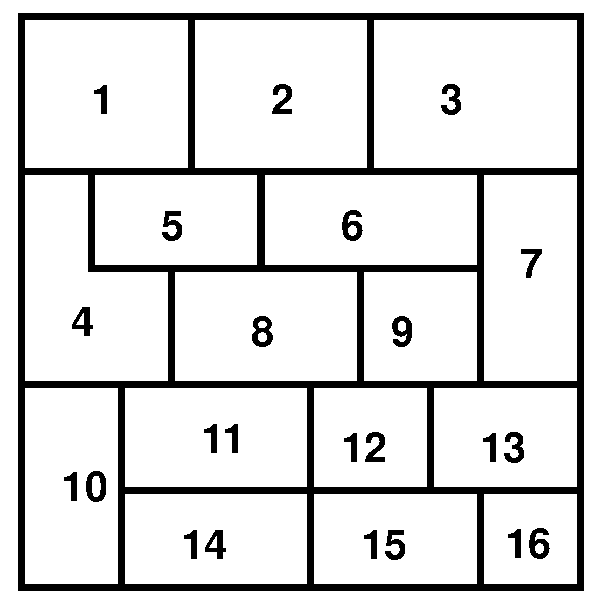
\includegraphics[width=0.5\textwidth]{SetCoveringProblemFig.pdf}
\end{center}

\begin{enumerate}
\item The city wants to build hospitals to service Annapolis. They want to make sure every district either contains a hospital, or is adjacent to another district containing a hospital. Formulate a concrete model that will allow them to make sure every district is serviced by a hospital while building the minimum number of hospitals.
\item Convert your concrete model from part 1 into an abstract model \emph{Hint: It may be helpful to define some extra sets that aren't directly in the problem or use the adjacency matrix idea from class}.
\end{enumerate}

\newpage

\section{Part 2: Logical Constraints}

Mazda's is considering opening a new plant in the US. They are considering manufacturing either Mazda3 (clearly the best), Mazda6, or Mazda Miatas. The table below shows the amount of each resource required for each type of car.

\begin{center}
\begin{tabular}{|c|c|c|c|}
\hline
            & \multicolumn{3}{|c|}{Type of Car} \\
Resource    & Mazda3  & Mazda6 & Mazda Miata \\ \hline
Steel (tons)& 2       & 3      & 1.5 \\
Labor hours & 30      & 40     & 25 \\ \hline
\end{tabular}
\end{center}

The plant can obtain 6000 tons of steel and 60,000 hours of labor. The profit of a Mazda3 is \$2000, a Mazda6 is \$3000, and a Mazda Miata is \$1500. Suppose the demand of each type of car is unlimited.

\begin{enumerate}[resume]
\item Formulate a concrete model whose solution will tell Mazda how to produce cars in order to maximize profit.
\item Suppose that management has decided that it is not worthwhile to produce Mazda Miatas unless you produce at least 1000 of them.	Modify your concrete model to reflect this new constraint. \emph{Hint: Convert this to an either/or constraint in words/math then write it as a constraint}.
\item Management has found a new machine that reduces the labor hours required for each car as follows: Mazda3 28 hours, Mazda6 35 hours, Mazda Miata 22 hours. The new machine costs \$100,000 if they decide to purchase it. Modify your concrete model to help Mazda decide if they should purchase this new machine.
\end{enumerate}

\end{document}
